\section{Оптические явления на границе раздела изотропных диэлектриков. Соотношения амплитуд падающей, отраженной и преломленной волн (формулы Френеля). Изменение фазы волны при отражении. Энергетические коэффициенты отражения и пропускания света. Коэффициент отражения для естественного света.}

% Дописать про изменение фазы волны при отражении -- вроде бы было в Овчинкине (семинары)?

% Коэффициент отражения -- ?????

При падении плоской волны на границу раздела двух изотропных диэлектриков, появляется две волны: преломленная (которая проходит границу раздела сред) и отраженная (не проходит), которые создаются за счет колебаний в диэлектриках, возбуждаемых падающей волной. Сразу быстро получим законы отражения и преломления.

\subsection{Законы отражения и преломления}

Пусть падающая волна имеет следующий вид:

\begin{equation*}
\vec{E} = \vec{E}_0 \cdot e^{-i (\omega t - \vec{k} \cdot r)}
\end{equation*}

В таком случае, из-за того, что колебания являются вынужденными, мы можем сказать, что $\omega = \omega_r = \omega_t$.

Кроме того, как мы знаем из курса электричества, существует уравнение на граничное условие для вектора $E$, которое в нашем случае принимает вид (для тангенциальных компонент):

\begin{equation*}
E_\tau + E_{r\tau} = E_{t\tau}
\end{equation*}

Возьмем любую точку на линии границы сред. В таком случае:

\begin{equation*}
A_1 e^{i \vec{k} \vec{x}} + B_1 e^{i \vec{k}_r \vec{x}} = C_1 e^{i \vec{k}_t \vec{x}}
\end{equation*}

Это в свою очередь значит, что должны быть равны между собой величины, стоящие в показателе экспоненты. С учетом того, как мы ввели углы, получаем:

\begin{equation}
k\sin\phi = k_r \sin \phi_r = k_t \sin\phi_t
\label{eq:reflection_and_refraction}
\end{equation}

При этом, как мы знаем, $k$ зависит от свойств среды, поэтому для падающей волны и отраженной:

\begin{equation*}
k = k_r = \frac{w}{c} \sqrt{\mu \epsilon}
\end{equation*}

А для преломленной:

\begin{equation*}
k_t = \frac{w}{c} \sqrt{\mu'\epsilon'}
\end{equation*}

Тогда из уравнения \ref{eq:reflection_and_refraction} получаем:

\begin{align*}
&\phi = \phi_r\\
&\frac{\sin\phi_t}{\sin\phi} = \frac{k}{k_t} = \frac{\sqrt{\epsilon\mu}}{\sqrt{\epsilon'\mu'}} = \frac{n}{n'}
\end{align*}

\subsection{Коэффициенты Френеля}

Разложим падающую волну $\vec{E}$ по двум составляющим: в плоскости, параллельной плоскости рисунка, и в плоскости, перпендикулярной ($E_\parallel$ и $E_\perp$ соответственно). Мы имеем следующие граничные условия:

\begin{align*}
&E_\tau + E_{r\tau} = E_{t\tau}\\
&H_\tau + H_{r\tau} = H_{t\tau}
\end{align*}

Мы также знаем соотношение, связывающее между собой $H$ и $E$: $H = \sqrt{\epsilon}E$ (пренебрегаем магнитными свойствами сред и считаем $\mu = 1$, а также не забываем, что $\vec{H} \perp \vec{E}$). Также вспоминаем, что $n = \sqrt{\epsilon}$. Тогда граничные условия принимают вид (с учетом проекций, см. рисунок):

\begin{figure}[H]
	\centering
	\subfigure[]{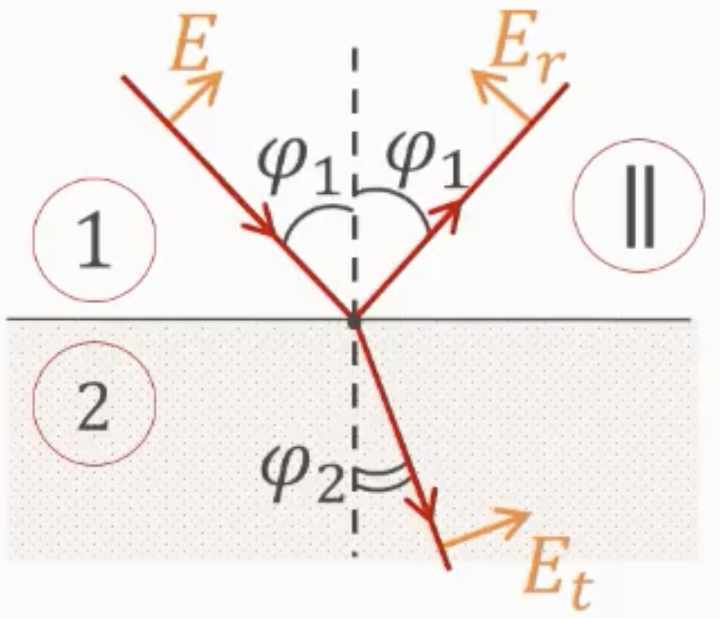
\includegraphics[width=0.48\linewidth]{11_1}
	}
	\subfigure[]{
	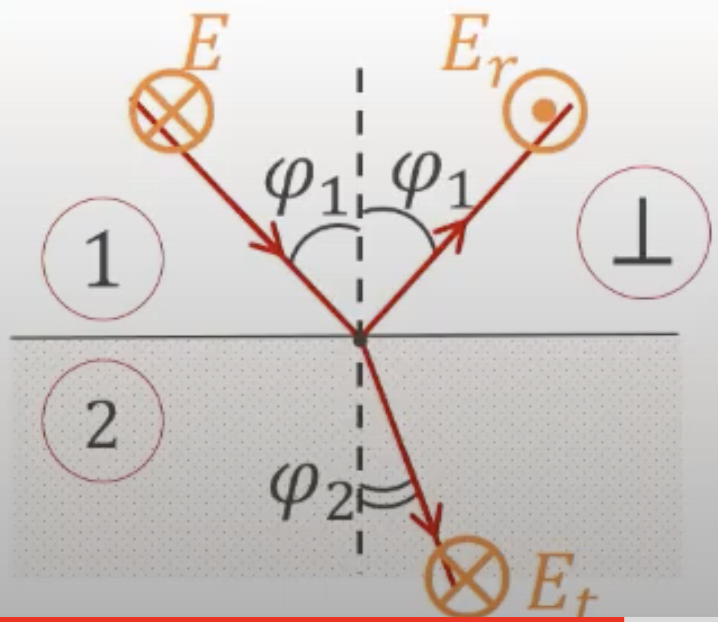
\includegraphics[width=0.48\linewidth]{11_2}
}
\end{figure}

\begin{align*}
&\begin{cases}
&E\cos\phi_1 - E_r\cos\phi_1 = E_t\cos\phi_2\\
&n_1 E + n_1 E_r = n_2 E_t\\
&\dfrac{\sin\phi_1}{\sin\phi_2} = \dfrac{n_2}{n_1}
\end{cases}
\quad &\text{--- для параллельной}\\
&\begin{cases}
&E - E_r = E_t\\
&n_1 E \cos\phi_1 + n_1 E_r \cos\phi_1 = n_2 E_t \cos\phi_2\\
&\dfrac{\sin\phi_1}{\sin\phi_2} = \dfrac{n_2}{n_1}
\end{cases}
\quad &\text{--- для перпендикулярной}\\
\end{align*}

Решив эту систему уравнений, мы получаем следующее:

\begin{align*}
&\begin{cases*}
E_r = \dfrac{\tg(\phi_1 - \phi_2)}{\tg(\phi_1 + \phi_2)}E\\
E_t = \dfrac{2\sin\phi_2\cos\phi_1}{\sin(\phi_1 + \phi_2) \cos(\phi_1 - \phi_2)}E
\end{cases*}
\quad &\text{--- для параллелльной}\\
&\begin{cases*}
E_r = \dfrac{\sin(\phi_2 - \phi_1)}{\sin(\phi_1 + \phi_2)}E\\
E_t = \dfrac{2\sin\phi_2\cos\phi_1}{\sin(\phi_1 + \phi_2)}E
\end{cases*}
\quad &\text{--- для перпендикулярной}
\end{align*}

Можно сразу же ввести энергетические коэффициенты отражения и пропускания света:

\begin{align*}
R_\parallel = \left(\frac{E_r}{E}\right)^2 = \frac{\tg^2\left(\phi_1 - \phi_2\right)}{\tg^2(\phi_1 + \phi_2)} \qquad T_\parallel = 1 - R_\parallel\\
R_\perp = \left(\frac{E_\perp}{E}\right)^2 = \frac{\sin^2(\phi_2 - \phi_1)}{\sin^2(\phi_2 + \phi_1)} \qquad T_\perp = 1 - R_\perp
\end{align*}